\id{ҒТАМР 20.23.17}{https://doi.org/10.58805/kazutb.v.4.25-602}

\begin{articleheader}
\sectionwithauthors{Д.К.Даркенбаев, Г.Ж.Жакшиликова, Н.О.Мекебаев}{БІЛІМ БЕРУГЕ АРНАЛҒАН АҚПАРАТТЫҚ ЖҮЙЕ ӘЗІРЛЕУ}

{\bfseries \textsuperscript{1}Д.К.Даркенбаев\textsuperscript{\envelope },
\textsuperscript{2}Г.Ж.Жакшиликова, \textsuperscript{2}Н.О.Мекебаев}
\end{articleheader}

\begin{affiliation}
\textsuperscript{1}Әл-Фараби атындағы қазақ ұлттық университеті, Алматы,
Қазақстан,

\textsuperscript{2}Қазақ ұлттық қыздар педагогикалық университеті,
Алматы, Қазақстан

\raggedright {\bfseries \textsuperscript{\envelope }}Корреспондент-автор: dauren.kadyrovich@gmail.com
\end{affiliation}

Қазіргі ақпараттық технологиялардың дамуынан туындаған білім беру
процесіндегі өзгерістер, білім беру саласындағы өте өзекті мәселелердің
бірі болып табылады. Білім беру үшін ақпараттық жүйелерді дамытудың
маңыздылығы, олардың функциялары, соның ішінде оқу процесін басқару,
деректерді сақтау және қашықтықтан оқытуды ұйымдастыру, өз кезеңінде
оқытуды білім алушылар мен педагогтардың қажеттіліктеріне бейімдеу
арқылы қол жетімді және тиімді екенін атап өтеді. Мақалада білім беру
мекемелерінің ерекшеліктері мен білім алушылардың талаптарын ескеретін
ақпараттық жүйелерді мұқият жобалау қажеттілігі зерттелген. Жүйелердің
сенімділігі, қауіпсіздігі және ыңғайлылығы сияқты негізгі аспектілер,
виртуалды және кеңейтілген шындық сияқты заманауи білім беру
технологиялары және олардың оқытудың интерактивтілігіне әсері де
салыстырыла талданған. Талдау нәтижесінде ақпараттық жүйелерге қойылатын
негізгі талаптар және олардың оқу процесін қарқындатудағы рөлі
ерекшеленеді. Мақалада цифрлық трансформация жағдайында білім беру
мекемелерінің алдында тұрған өзекті міндеттер талқыланған, қазіргі
заманғы технологияларды бағдарлай алатын ақпараттық сауатты мамандарды
даярлау мәселелері зерттелген.Зерттеу барысында білім беру жүйелерін
жобалаудың теориялық негіздері талданып, ақпараттық жүйе құруға талаптар
мен техникалық шешімдер қабылдау мәселелері сараланған. Бұл жүйе білім
алушылардың оқыту процесін жеңілдетіп, білім алушылардың интеллектуалды
дамуына оң ықпал етеді.Мақала авторлары алдағы уақытта зерттеу
жұмыстарын әрі қарай жалғастыруды жоспарлап отыр.

{\bfseries Түйін сөздер:} ақпарат, жүйе, технология, диаграмма, компьютер,
модель, өңдеу, сервер.

\begin{articleheader}
{\bfseries РАЗРАБОТКА ИНФОРМАЦИОННОЙ СИСТЕМЫ ДЛЯ ОБРАЗОВАНИЯ}

{\bfseries \textsuperscript{1}Д.К.Даркенбаев\textsuperscript{\envelope },
\textsuperscript{2}Г.Ж. Жакшиликова, \textsuperscript{2}Н.О.Мекебаев}
\end{articleheader}

\begin{affiliation}
\textsuperscript{1}Казахский национальный университет имени аль-Фараби,
Алматы, Казахстан,

\textsuperscript{2}Казахский национальный женский педагогический
университет,Алматы, Казахстан,

е-mail:
\href{mailto:dauren.kadyrovich@gmail.com}{\nolinkurl{dauren.kadyrovich@gmail.com}}
\end{affiliation}

Изменения в образовательном процессе, связанные с развитием современных
информационных технологий, являются одной из наиболее актуальных тем в
образовании. Важность разработки информационных систем для образования
обуславливает их такие явления, как управление научным процессом,
хранение данных и организация дистанционного обучения, которые
становятся более доступными и эффективными благодаря адаптации к
потребностям образования и образования. В статье обоснована
необходимость информационного проектирования с системами государственных
учреждений и запроса обучающихся. Внимание также уделяется таким
аспектам, как надежность, безопасность и удобство использования систем,
а также современным образовательным технологиям, таким как виртуальная и
дополненная реальность, и их перспективность в интерактивности текущего
процесса. По результатам анализа определяются основные требования к
информационным системам и их важная роль в ускорении обучения.
Рассматриваются задачи, стоящие перед образовательными преобразованиями
в условиях цифровой трансформации, а также вопросы подготовки
специалистов, способных эффективно работать с современными технологиями.
В ходе анализа разрабатываются теоретические основы проектирования
образовательных систем, определяются требования к созданию
информационных систем и обсуждаются сложности с использованием
технических решений. Эти системы способствуют облегчению нынешних
процессов и положительно влияют на интеллектуальное развитие учащихся.
Авторы планируют продолжить свои исследования в данной области.

{\bfseries Ключевые слова:} информация, система, технология, диаграмма,
компьютер, модель, обработка, сервер.

\begin{articleheader}
{\bfseries DEVELOPMENT OF AN INFORMATION SYSTEM FOR EDUCATION}

{\bfseries \textsuperscript{1}D.K.Darkenbayev\textsuperscript{\envelope },}
{\bfseries \textsuperscript{2}G.Zh. Zhakshilikova,}
{\bfseries \textsuperscript{2}N.O.Mekebayev,}
\end{articleheader}

\begin{affiliation}
\textsuperscript{1}Al-Farabi Kazakh National University, Almaty,
Kazakhstan,

\textsuperscript{2}Kazakh National Women' s Pedagogical
University, Almaty, Kazakhstan,

е-mail: dauren.kadyrovich@gmail.com
\end{affiliation}

Changes in the educational process associated with the development of
modern information technologies are one of the most pressing topics in
education. The importance of developing information systems for
education determines such phenomena as scientific process management,
data storage and distance learning organization, which become more
accessible and effective due to adaptation to the needs of education and
learning. The article substantiates the need for information design with
the systems of state public institutions and the request of students.
Attention is also paid to such aspects as reliability, security and
usability of systems, as well as modern educational technologies such as
virtual and augmented reality and their prospects in the interactivity
of the current process. Based on the analysis, the main requirements for
information systems and their important role in accelerating learning
are determined. The challenges facing educational transformations in the
context of digital transformation are considered, as well as the issues
of training specialists who can effectively work with modern
technologies. During the analysis, the theoretical foundations of
designing educational systems are developed, the requirements for the
creation of information systems are determined and the difficulties in
using technical solutions are discussed. These systems help to
facilitate current processes and have a positive effect on the
intellectual development of students. The authors plan to continue their
research in this area.

{\bfseries Keywords:} information, system, technology, diagram, computer,
model, processing, server.

\begin{multicols}{2}
{\bfseries Кіріспе}.Ақпараттық технологиялардың қарқынды даму дәуірінде
білім айтарлықтай өзгерістерге ұшырады. Дәрістер мен қағаз
материалдарына негізделген дәстүрлі оқыту әдістері цифрлық
технологияларды қолдануға негізделген интерактивті және тиімді
тәсілдерге мүмкіндік береді. Бұл тұрғыда білім беру үшін ақпараттық
жүйелерді әзірлеу аса маңызды. Ақпараттық жүйелер білім беру процесін
өзгерте алады, оны қол жетімді, тиімді және білім алушылар мен
педагогтардың қажеттіліктерін қамтамасыз ете алады.

Білім берудегі ақпараттық жүйелердің қажеттілігі оқу процесін басқарудан
және білім алушылардың деректерін сақтаудан бастап, білім беру
ресурстарына қол жетімділікті қамтамасыз етуге және қашықтықтан оқытуды
ұйымдастыруға дейінгі көптеген функцияларды қамтиды. Бұл оқу орнын
басқаруды оңтайландыруға ғана емес, сонымен қатар білім алушылардың жеке
қажеттіліктеріне бейімдеу арқылы білім сапасын жақсартуға мүмкіндік
береді.Алайда, тиімді ақпараттық жүйені құру дамудың барлық кезеңдерінде
мұқият қарауды қажет етеді. Ақпараттық жүйені жобалау барысында, білім
беру мекемесінің ерекшелігі, білім алушылардың талаптары, технологиялар
мен педагогика тенденциялары сияқты факторларды ескеру қажет. Талаптарды
талдау кезеңінде жүйенің олардың қажеттіліктері мен мүмкіндіктерін
қанағаттандыруы үшін білім алушыларға не қажет екенін түсіну маңызды.
Ақпараттық жүйенің архитектурасын жобалауда басқа платформалармен
интеграциялау мүмкіндігін ескеру керек, бұл әсіресе білім беру
стандарттары мен технологияларын үнемі жаңартып отыру жағдайында
маңызды.

Ақпараттық жүйе (АЖ) -- басқару немесе шешім қабылдау процесінде
қолданылатын ақпаратты жинау, сақтау, жинақтау, іздеу және беру жүйесі.
Ол әдетте ақпараттық-анықтамалық қорды (құжаттар, мәліметтербазасы,
ақпараттыққоймалар), ақпаратты өңдеу және жүйемен байланыс тілін,
ақпарат тасымалдаушыларды, сондай-ақ жүйенің жұмыс істеуін қамтамасыз
ететін модельдер кешенін қамтиды.

Ақпараттық жүйе (АЖ) -- деректерді автоматтандырылған жинау, өңдеу және
басқару үшін қолданылатын техникалық және бағдарламалық құралдардың,
әдістердің және қызмет көрсету персоналының өзара байланысты жиынтығы
{[}1{]}. Ақпараттық және коммуникациялық технологиялар білім беруді әр
түрлі деңгейде өзгертеді. Білім беру қызметіндегі жаңа басымдықтар білім
беру ұйымдарының басқару қызметін ақпараттық қолдау болып
табылады{[}2{]}. Мақалада жазу барысында зерттеліп жобаланған жүйе білім
берудің цифрлық трансформациясы білім беру мекемесін ақпараттандырудан
әлдеқайда асып түседі. Цифрлық білім берудің белгісі
ақпараттық-коммуникациялық технологиялар (бұдан әрі АКТ технологиялар)
негізінде кешенді көп деңгейлі интеграцияланған орта екенін атап өту
қажет: білім беру контентін әзірлеу және басқару, әртүрлі деңгейдегі
ақпараттық жүйелермен интеграциялау, білім алушылардың қажеттіліктеріне
сәйкес білім беру траекторияларын құру {[}3{]}. Білім беру саласына
ақпараттық жүйені енгізу білім алушыларды оқыту қажеттілігімен қатар
жүреді, бұл жұмыстың жаңа форматына біркелкі көшуді қамтамасыз етеді.
Сонымен қатар, жүйені іске қосқаннан кейін бақылау және қолдау оның ұзақ
мерзімді тиімділігін қамтамасыз етуде маңызды рөл атқарады{[}4{]}.

Білім беру жүйесіндегі ақпараттық жүйенің мақсаты:

\begin{itemize}
\item
  білім беру тиімділігін арттыру;
\item
  білім берудің икемділігі мен қолжетімділігін арттыру;
\item
  ақпараттық мәдениетті дамыту {[}5{]}.
\end{itemize}

Ақпараттық жүйені құрудың маңыздылығы қазіргі білім беру мекемелерінің
басты міндеттерінің бірі - білім беру үдерісіне цифрлық ортаны енгізуге
бағытталған педагогтардың цифрлық сауаттылығын дамыту қажеттілігімен
айқындалады. Цифрлық орта педагогтар мен білім алушыларға жаңа бағыт пен
үнемі біліктілікті көтеріп отуды талап ететіні белгілі.Оқытушы цифрлық
технологияларды қолдана отырып, компьютерлік бағдарламалау, ақпаратты
іздеу, алмасу және коммуникация дағдыларын меңгеріп, үнемі жетілдіріп
отыруы қажет {[}6{]}.

{\bfseries Материалдар мен тәсілдер.} Қазіргі білім -- білім мен заманауи
технологиялардың интеграциясы {[}7{]}. Білім және заманауи
технологиялардың интеграциясы педагогпен білім алушылардың арасындағы
оқытумен өзара әрекеттесу тәсілдерін өзгертетін динамикалық және
көпқырлы жүйе. Виртуалды шындық (VR) және кеңейтілген шындық (AR) сияқты
технологиялар интерактивті және иммерсивті білім беру орталарын құруға
мүмкіндік береді. Төменде көрсетілген суретте (1-сурет) ақпараттық жүйе
негізінде басқарылатын жалпы білім беретін орындардың білім беру
процесінің жалпы моделі бейнеленген.

Білім беру процесінің жалпы моделі -- білім беру процесінің әртүрлі
компоненттерінің ақпараттық технологияларды қолдану арқылы бір-бірінен
қалай әрекеттесеттінін сипаттайтын құрылым. Модель ақпараттық жүйелермен
бірге білім беру процесіне қатысушылар арасындағы оқыту, басқару және
өзара әрекеттесу процесін ұйымдастыруға және оңтайландыруға ықпал ету
көрінісін бейнелеп тұр.

Білім беруге негізделген ақпараттық жүйелерге қойылатын талаптар:

1. Ақпаратты өңдеудің толықтығы -- қажетті ақпаратпен қажетті көлемде
қамтамасыз ету.

2. Сапа -- жүйенің берілген функцияларды орындауға жарамдылық дәрежесі.

3. Ақпараттық жүйеге деген сенімділік -- техникалық құралдары мен
бағдарламалық жасақтамасының арасында қателіктердің туындамауы.

4. Ақпараттық жүйенің қауіпсіздігі.

5. Пайдаланудың ыңғайлылығы -- әзірленетін жүйеде тиісті бөлімшенің
ерекшеліктерін, онда өңделетін ақпарат пен әзірленетін құжаттардың
құрамын, мазмұны мен нысандарын барынша есепке алуды талап ету.

6. Модульдік -- білім беруге арналған ақпараттық жүйенің элементтерін
салыстырмалы түрде тәуелсіз және функционалды түрде аяқталған
стандартты бөліктерден-модульдерден құру мүмкіндігі.

7. Сүйемелдеу -- сапаны жақсарту мүддесінде жүйенің ұзақ мерзімді
пайдалануға және жетілдіруге жоғары дәрежеде бейімделуін қамтамасыз
ету.

Білім берудің заманауи ақпараттық жүйелері оқыту және оқу процесін
басқаруды айтарлықтай өзгертеді. Осы негізде білім беруге арналған
ақпараттық жүйені бірнеше категорияларға бөліп қарастырып, категорияға
сәйкес төмендегі 1-кестеде мысал ретінде бірнеше ақпараттық жүйелер
көрсетілген.
\end{multicols}

\begin{figure}[H]
	\centering
	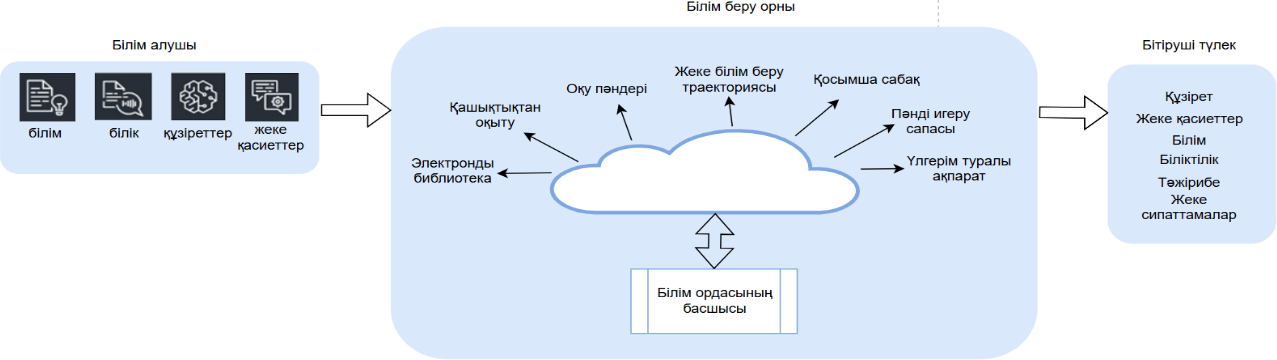
\includegraphics[width=0.8\textwidth]{media/ict/image99}
	\caption*{1-сурет. Білім беру процесінің жалпы моделі}
\end{figure}

\begin{longtable}[c]{|lllllll|}
\caption*{1-кесте. Білім беру арналған ақпараттық жүйелер} \\
\hline
\multicolumn{7}{|c|}{Оқытуды басқару жүйесі} \\ \hline
\endfirsthead
%
\endhead
%
\multicolumn{3}{|c|}{Атауы} &
  \multicolumn{1}{c|}{Артықшылығы} &
  \multicolumn{3}{c|}{Кемшілігі} \\ \hline
\multicolumn{3}{|p{2cm}|}{Moodlе} &
  \multicolumn{1}{p{0.4\textwidth}|}{\begin{tabular}{@{}p{0.4\textwidth}@{}}Жаңа курс құру\\  Оқу процесін басқару\\  Мультимедиялық материалдар\\  Форумдар мен талқылаулар\\  Онлайн тестілеу\\  Оқушы үлгерімін бағалау\end{tabular}} &
  \multicolumn{3}{p{0.4\textwidth}|}{\begin{tabular}{@{}p{0.4\textwidth}@{}}Платформаны орнату қиындығы\\  Платформаны жаңарту кезіндегі қиындықтар\\  Пайдаланушы интерфейсі күрделі\\  Шектеулі интеграциялар\\  Техникалық қиындықтар\end{tabular}} \\ \hline
\multicolumn{3}{|p{2cm}|}{Canvas} &
  \multicolumn{1}{p{0.4\textwidth}|}{\begin{tabular}{@{}p{0.4\textwidth}@{}}Интуитивті интерфейс\\  Курстардың икемділігі\\  Бағалау және кері байланыс\\  Басқа платформалармен интеграция\end{tabular}} &
  \multicolumn{3}{p{0.4\textwidth}|}{\begin{tabular}{@{}p{0.4\textwidth}@{}}Орнатудың қиындылығы\\  Тегін нұсқаның шектеулі мүмкіндік-тері\\  Оқу уақыты\end{tabular}} \\ \hline
\multicolumn{7}{|c|}{Онлайн оқыту платформасы} \\ \hline
\multicolumn{3}{|p{2cm}|}{Coursera} &
  \multicolumn{1}{p{0.4\textwidth}|}{\begin{tabular}{@{}p{0.4\textwidth}@{}}Технологияның әртүрлі бағыттары бағыттары бойынша көпетеген курстар ұсынады\\  Белгілі университеттер мен компаниялардан сертификаттар мен дипломдар алу мүмкіндігі\\  Белсенді оқытуға ықпал ететін бейне жазбалар мен тесттер, тәжірибелік сабақтар\end{tabular}} &
  \multicolumn{3}{p{0.4\textwidth}|}{\begin{tabular}{@{}p{0.4\textwidth}@{}}Көптеген курстар ақылы\\  Сапалы және сапасыз курстардың санының көптігі\\  Оқытушылармен тарапынан жеткілікті қолдаудың болмағаны\end{tabular}} \\ \hline
\multicolumn{3}{|p{2cm}|}{edX} &
  \multicolumn{1}{l|}{\begin{tabular}{@{}p{0.4\textwidth}@{}}Беделді университеттердің курстары\\  Көптеген курстарды тегін оқу мүмкіндігі\\  MicroMasters және Professional Certificates\\  Іс жүзінде қолдануға мүмкіндік беретін тәжірибелік тапсырмалар\end{tabular}} &
  \multicolumn{3}{l|}{\begin{tabular}{@{}p{0.4\textwidth}@{}}Курстардың күрделілігі\\  Шектеулі интерактивті курстар\\  Платформадағы техникалық мәселелер\end{tabular}} \\ \hline
\multicolumn{7}{|c|}{Бірлескен жұмыс құралдары} \\ \hline
\multicolumn{2}{|p{2cm}|}{Google workspace} &
  \multicolumn{4}{p{0.4\textwidth}|}{\begin{tabular}{@{}p{0.4\textwidth}@{}}Gmail, Google Docs, Sheets, Slides, Drive жүйелермен бір уақытта жұмыс жасау мүмкіндігі\\  Бірнеше пайдаланушыға құжаттарды бір уақытта өңдеуге мүмкіндік беруі\end{tabular}} &
  \begin{tabular}{@{}p{0.4\textwidth}@{}}Интернетке тәуелділік\\  Деректердің құпиялылығы\\  Ақылы функцияларда мүмкіндіктер көптігі\end{tabular} \\ \hline
\multicolumn{2}{|p{2cm}|}{Microsoft Teams} &
  \multicolumn{4}{l|}{\begin{tabular}{@{}p{0.4\textwidth}@{}}Басқа Microsoft құралдарымен интегра­ция\\  Бірлескен мүмкіндіктер\\  Командалар мен сыныптарды басқару\\  Бейне конференциялармен сыныптарды басқару\end{tabular}} &
  \begin{tabular}[c]{@{}l@{}}Платформаны орнатудың қиындығы\\  Тегін нұсқаның шектеулі мүмкіндік­тері\\  Пайдаланушы интерфейсінің күрделі­лігі\\  Деректерді қорғау және құпиялылық\end{tabular} \\ \hline
\multicolumn{7}{|c|}{Виртуальды және толықтырылған шындық} \\ \hline
\multicolumn{1}{|p{2cm}|}{{Google Expeditions}} &
  \multicolumn{4}{l|}{\begin{tabular}{@{}p{0.4\textwidth}@{}}Көптеген виртуальды турлармен экскурсияларға мүмкіндік\\  Интуитивтіинтерфейс\\  Мазмұнныңәртүрлілігі\\  виртуалдынысандарменөзараәрекеттесу мүміндігі\end{tabular}} &
  \multicolumn{2}{l|}{\begin{tabular}{@{}p{0.4\textwidth}@{}}Жақсы интернет жүйесінің болуын қажет етеді\\  Виртуальды мүмкіндіктердің аздығы\\  Техникалық ақаулардың орын алу мүмкіндігі\end{tabular}} \\ \hline
\multicolumn{1}{|p{2cm}|}{zSpace} &
  \multicolumn{4}{l|}{\begin{tabular}{@{}p{0.4\textwidth}@{}}Тақырыптарды кеңінен түсінуге ықпал ететін виртуальды және толықтырылған шығдық тапсырмалары\\  Тақырыптардың кең ауқымы\end{tabular}} &
  \multicolumn{2}{l|}{\begin{tabular}{@{}p{0.4\textwidth}@{}}Платформаның оқу орындары үшйн қымбаттылығы  \\  Аппараттық және бағдарламалық жасақтаманы орнату қиындығы\\  Шектеулі қолжетімділік\end{tabular}} \\ \hline
\end{longtable}

\begin{multicols}{2}
Бұл технологиялар білім беруді жаңа мазмұнмен толтыру үшін, білім
алушылардың шығармашылығы мен шығармашылық қабілетін дамытатын оқытудың
жаңа формалары мен әдістерін қолдану үшін қолданылған кезде тиімді
болады.

Ашық білім беру жүйелерін дамыту білім беру мекемелерінің әлемдік білім
беру қызметтері нарығындағы бәсекелестігінің жаңа нысандарын тудырады.

Қазіргі білім саласы заманауи технологиялардың дамуымен, интернеттің
қолжетімділігінің арқасында айтарлықтар өзгерістерге ұшырауда. Білім
саласында қолданысқа ие платформалардың функциональдылығы барлық білім
алушыларға бір уақытта бірнеше адаммен байланыс орнатуға, ақпараттық
ресурстарға, конференциялар мен вебинарларға қатысуға, туындаған
мәселеге байланысты онлайн пікір таластырулар ұйымдастыруға мүмкіндік
береді (2-сурет).

Ақпараттық жүйені әзірлеу білім беру процесін ұйымдастырудың заманауи
тәсілінің ерекшелігін көрсетеді, бұл білім алушының жаңа білімді өз
бетінше алу қабілетін қалыптастыруға және оларды болашақ кәсіби
қызметтің міндеттерін шешуге қолдануға дайын болуға бағытталған қол
жетімді интерактивті білім беру ортасын құруды қамтиды {[}8{]}. Бүгінгі
таңда білім берудің әртүрлі салаларына ақпараттық жүйелерді енгізу
кезінде келесі міндеттер орындалуы тиіс. Білім алушының интеллектуалды
тұлғасын дамыту, жеке тұлғаны ақпараттық қоғам жағдайында жайлы өмір
сүруге бейімдеу, ақпаратты қабылдау және өңдеу қабілеттерін дамыту,
әлеуметтік дағдыларды жетілдіру, сондай-ақ қойылған міндетті тез талдау
және оңтайлы шешім табу мүмкіндігі {[}9{]}.
\end{multicols}

\begin{figure}[H]
	\centering
	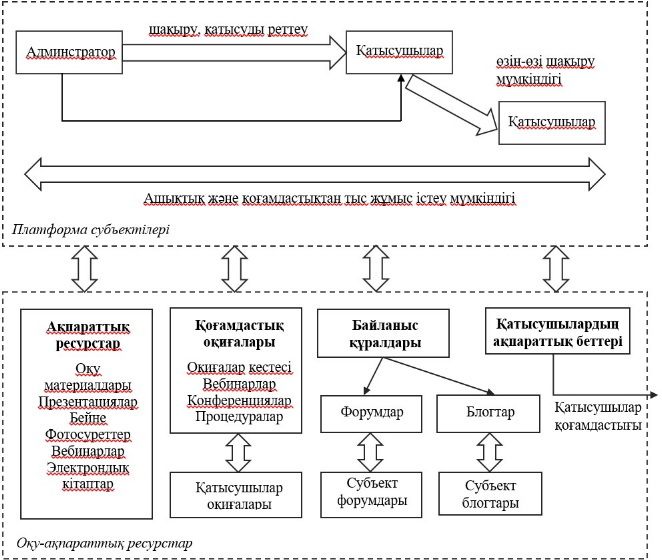
\includegraphics[width=0.7\textwidth]{media/ict/image100}
	\caption*{2-сурет. Білім беруге арналған ақпараттық жүйенің
фукнционалдылығы}
\end{figure}

\begin{multicols}{2}
Оқу-тәрбие процесін қарқындату. Бұл тұжырымдама білім алушының алған
білім сапасын жоғалтпай және оқу ұзақтығын өзгертпестен білім алушыға
берілетін ақпарат көлемін ұлғайтуды білдіреді. Заманауи технологияларға
бағдарланған және болашақта еңбек нарығында өзін сенімді сезінуге
қабілетті ақпараттық сауатты адамды дайындау {[}10{]}.

{\bfseries Нәтижелер мен талдау.}Зерттеу барысында білім беру мекемелері
үшін ақпараттық жүйелерді әзірлеуде қолданылатын ағымдағы
тенденцияларды, әдістер мен құралдарға талдау жүргізілді.

Білім беруге арналған ақпараттық жүйелер мынадай қызмет түрлерін жүзеге
асыру мүмкіндігін қамтамасыз етеді:

\begin{itemize}
\item
  білім беру процесін жоспарлайды;
\item
  білім беру процесінің барысын және білім беру бағдарламаларын игеру
  нәтижелерін белгілейді;
\item
  білім алушылар арасындағы өзара іс -- қимыл, оның ішінде-интернет
  желісі арқылы қашықтықтан оқытады;
\item
  білім беру қызметін басқару міндеттерін шешу үшін білім беру процесі
  барысында қалыптастырылатын деректерді пайдалану мүмкіндігін
  жоғарылатады;
\item
  білім алушылар интернет желісінің ақпараттық білім беру ресурстарына
  бақыланатын қолжетімділікті арттырады;
\item
  білім беру мекемесінің білім беру саласындағы басқаруды жүзеге
  асыратын органдармен, сондай-ақ басқа да білім беру мекемелерімен және
  ұйымдарымен өзара іс-қимылды жеңілдетеді.
\end{itemize}

Білім алушылар мен педагогтардың өзара байланысын визулизациялауға
көмектесу үшін ақпараттық жүйенің архитектурасы жобаланды. Төменде
3-суртетте көрсетілген.
\end{multicols}

\begin{figure}[H]
	\centering
	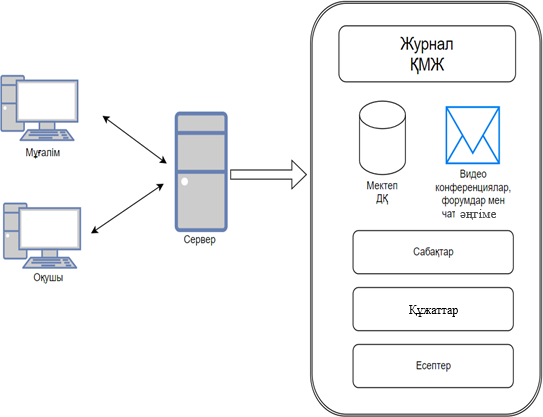
\includegraphics[width=0.6\textwidth]{media/ict/image101}
	\caption*{3-сурет. Ақпараттық жүйе архитектурасы}
\end{figure}

\begin{figure}[H]
	\centering
	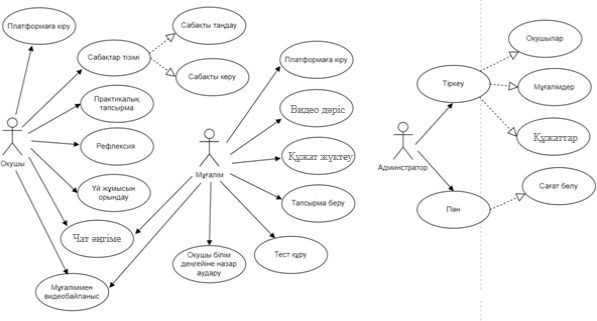
\includegraphics[width=0.7\textwidth]{media/ict/image102}
	\caption*{4-сурет. Use case диаграмма}
\end{figure}

\begin{multicols}{2}
Білім беруге арналған ақпараттық жүйенің архитектурасы білім беру
процесін қолдауға бағытталған компоненттердің құрылымдық сипаттамасы
және олардың өзара әрекеттесуі көруге көмектеседі (3-сурет). Ақпараттық
жүйенің әрбір бөлігін сипаттау үшін UML бірыңғай модельдеу тілі
қолданылды.

UML модельдеу тілі объектілерді, бизнес процестерді модельдеуге және
жүйелік жобалауға және ұйымдық құрылымдарды көрсетуге арналған
графикалық сипаттау тілі және ол бағдарламалаушыларға, жүйе
аналитиктеріне, дизайнерлерге жүйенің күрделі аспектілерін түсінуге
көмектеседі.UML тілінің басты мақсаты -- күрделі жүйелерді
визуализациялау және түсіну.

Білім беруге арналған ақпараттық жүйенің «Use case» диаграммасы --
ақпараттық жүйені жобалау процесінің бір бөлігі болып табылады және
жүйенің функционалдық талаптарын анықтау мен сипаттау үшін қолданылады.
Диаграмма -- ақпараттық жүйенің пайдаланушылармен қалай әрекеттесетінін
және оның қандай функцияларды орындайтынын көрсетеді (4-сурет).

Ақпараттық жүйенің белгілі бір сценарий шеңберінде объектілер немесе
компоненттер арасындағы өзара әрекеттесуді визуализациялауға реттілік
диаграммасын қолдандық (5-сурет). Реттілік диаграммасы пайдаланушылар
мен ақпараттық жүйенің өзара байланысын қалыптастыруға негіз болды.
\end{multicols}

\begin{figure}[H]
	\centering
	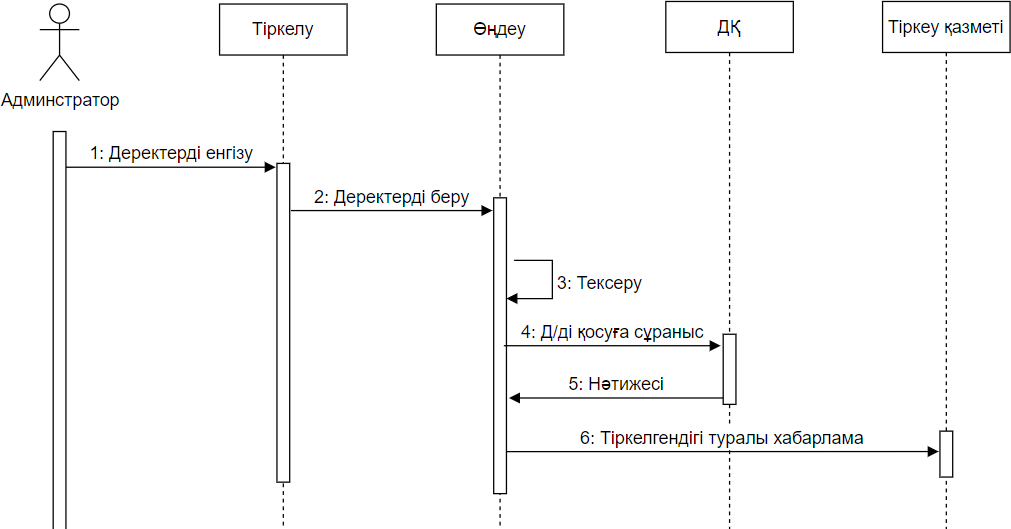
\includegraphics[width=0.7\textwidth]{media/ict/image103}
	\caption*{5-сурет. Ақпараттық жүйенің реттілік диаграммасы}
\end{figure}

\begin{multicols}{2}
Диаграмма жүйенің компоненттері арасындағы әрекеттер мен хабарламалар
тізбегін көрсету арқылы пайдалану процестерін егжей-тегжейлі көрсетуге
көмектеседі. Бұл use case диаграммаларында анықталған функциялардың
қалай жүзеге асырылатынын жақсы түсінуге мүмкіндік береді.

Білім беруге арналған ақпараттық жүйе өте күрделі және көп уақытты талап
ететін процесс. Білім беру саласы дамып келе жатқандықтан көптеген
процестер жаңашылдықты, жаңа технологиялар мен жаңа ресурстарды талап
етеді.

{\bfseries Қорытынды.} Мақалада білім беруге арналған ақпараттық жүйені
әзірлеу мәселесі зерттелген және оның білім беру саласында заманауи
білім беру процесін ұйымдастыруға қажетті құрал екені дәлелденген.
Ақпараттық жүйелерді білім саласында сәтті енгізу білім алушылардың да,
педагогтардың да қажеттіліктерін қанағаттандырады және білім берудің
тиімділігі мен икемділігін едәуір арттыруға мүмкіндік береді.

Жобаланған ақпараттық жүйенің негізгі артықшылықтары:

\begin{enumerate}[leftmargin=*]
\def\labelenumi{\arabic{enumi}.}
\item
  Оқытуды даралау. Жүйе білім алушының жеке қажеттіліктер мен
  қалауларына сәйкес материалды зерттеудің қарқыны мен дәйектілігін
  таңдай отырып, өздерінің білім беру траекториясын дербес құруға
  мүмкіндік береді.
\item
  Интерактивтілік және тәжірибелік фокус. Платформа білім алушылардың
  алған білімдері мен дағдыларын оқу процесінде белсенді қолдануға
  мүмкіндік беретін интерактивті жаттығулардың, тапсырмалардың және
  құралдардың кең ауқымын қамтиды.
\item
  Қашықтан және асинхронды өзара әрекеттесу. Білім алушылар теориялық
  материалды оқи алады, тапсырмаларды орындай алады және кезкелген
  педагогтан өздеріне ыңғайлы уақытта аудиториялық сабақтар шеңберімен
  шектелмей кері байланыс ала алады.
\item
  Үлгерім мониторингі және жеке қолдау. Жүйе білім алушылардың үлгерімін
  тиімді бақылауды, тапсырмаларды автоматтандырылған тексеруді және одан
  әрі оқыту бойынша жекелендірілген ұсыныстарды қамтамасыз етеді.
\end{enumerate}

Ақпараттық жүйені одан әрі жетілдіру оның функционалдық мүмкіндіктерін
кеңейтуге, басқа білім беру ресурстарымен интеграциялауға, сондай-ақ
әртүрлі оқу бағдарламалары мен білім беру ұйымдарының ерекшеліктеріне
бейімделуге бағытталуы мүмкін. Мұндай шешімдерді енгізу білім беруді
неғұрлым қолжетімді және тиімді етуге мүмкіндік береді.
\end{multicols}

\begin{center}
{\bfseries Әдебиеттер}
\end{center}

\begin{references}
1. G.T.Balakayeva,D.K.Darkenbayev, M.Zhanuzakov.Development of a software
system for predicting employee ratings // Informatyka, Autovatyka,
Pomiary w Gospodarce I Pchronie Srodowiska, 2023. -- Vol.13(3). -P.
121--124.DOI 10.35784/iapgos.3723

2. Ni Wayan Aprillia Pratiwi,Ida Bagus Surya Manuaba. The Effectiveness
Of A Concrete Media Assisted Project Based Learning Model On Students
' Science Competency // Journal of Education
Technology. -2020. -Vol.4(4). - P. 465-470.
\href{https://doi.org/10.23887/jet.v4i4.27112}{DOI
10.23887/jet.v4i4.27112}

3. Isa, W.A.R.W.M., Suhaimi, A.I.H., Noordin, N.~\emph{et al.} Hunger
hero mobile application: applying soft system methodology at a local
orphanage // International Journal of Information Technology. - 2023.
-Vol.15, -P.691--696. DOI 10.1007/s41870-022-01101-w

4. Ade Mukhfir Guswara, Wawan Purwanto. The Contribution of Google
Classroom Application and Motivation to The Learning Outcomes of Web
Programming //Journal of Education Technology. -2020. -Vol.4(4). - P.
424 - 432. \href{https://doi.org/10.23887/jet.v4i4.29896}{DOI
10.23887/jet.v4i4.29896}

5. G.T.Balakayeva, P.Ezhichelvan, M.K.Tursynkozha. Analysis Research and
Development of an Innovative Enterprise Digitalization System for
Remote Work // International Journal of Mathematics and Physics.-2022.
-Vol.13(1). -P.19-29.DOI 10.26577/ijmph.2022.v13.i1.02

6.D.Darkenbayev. BigData processing on the example of credit scoring
//Journal of problems in computer science and information technologies.
- 2023. -Vol.1.-P.50 -- 61. \href{https://doi.org/10.26577/1i32jpcsit2307}{DOI
10.26577/1i32jpcsit2307}

7.\href{https://link.springer.com/article/10.1007/s40593-024-00443-9\#auth-Yue-Huang-Aff1}{Yue
Huang},
\href{https://link.springer.com/article/10.1007/s40593-024-00443-9\#auth-Joshua-Wilson-Aff2}{Joshua
Wilson},
\href{https://link.springer.com/article/10.1007/s40593-024-00443-9\#auth-Henry-May-Aff2}{Henry
May}. Exploring the~Long‑Term Efects of~the~Statewide Implementation
of~an~Automated Writing Evaluation System on~Students' State Test ELA
Performance. // International Journal of Artifcial Intelligence in
Education. -2024. -Vol.34(3). -P. 1- 30. DOI 10.1007/s40593-024-00443-9

8.D.K.Darkenbayev, A.Altybay, Zh.Darkenbayeva, N.O.Mekebayev.
Intelligent Data Analysis on an Ana-lytical platform // Informatyka,
Autovatyka, Pomiary w Gospodarce I Pchronie Srodowiska. - 2024.
-Vol.14(1). - P. 119-122. DOI 10.35784/iapgos.5423

9.Schwab M., Strobelt H., Tompkin J., Fredericks C., Huff C., Higgins
D., Strezhnev A., Komisarchik M., King, G., \&Pfister H. An Education
System with Hierarchical Concept Maps // IEEE Transactions on
Visualization and Computer Graphics.- 2016. -Vol.22(9). -P. 2111- 2124.
\\DOI 10.1109/TVCG.2016.2598518

10.\emph{S}hi, D., Cui W., Huang D., Zhang H., \& Cao N.
Reverse-Engineering Information Presentations: Recov-ering Hierarchical
Grouping from Layouts of Visual Elements // Association for Computing
Machinery. - 2022. -Vol.1(1). - P.1-21. DOI 10.1007/s44267-023-00010-1
\end{references}

\begin{authorinfo}
\hspace{1em}\emph{{\bfseries Авторлар туралы мәліметтер}}

ДаркенбаевД.К. - PhD, әл-Фараби атындағы Қазақ ұлттық университетінің
доцент м.а., Алматы, Қазақстан, e-mail:\\
\href{mailto:dauren.kadyrovich@gmail.com}{\nolinkurl{dauren.kadyrovich@gmail.com}};

Жакшиликова Г.Ж. -Қазақ ұлттық қыздар педагогикалық университетінің
магистранты, Алматы, Қазақстан, e-mail: \\gulnur201801@gmail.com;

Мекебаев Н.О. - PhD, Қазақ ұлттық қыздар педагогикалық университетінің
қауымдастырылған профессор м.а., Алматы, Қазақстан, e-mail:
nurbapa@gmail.com

\hspace{1em}\emph{{\bfseries Information about the authors}}

D.Darkenbayev - PhD, Acting Associate Professor Al-Farabi Kazakh
National University,Almaty, Kazakhstan, e-mail:\\
\href{mailto:dauren.kadyrovich@gmail.com}{\nolinkurl{dauren.kadyrovich@gmail.com}};

G.Zhakshilikova - Master' s student, Kazakh National
Women' s Pedagogical University, Almaty,
Kazakhstan, e-mail: \\gulnur201801@gmail.com;

N.Mekebayev - PhD, Acting Associate Professor Kazakh National
Women' s Pedagogical University, Almaty,
\\Kazakhstan, e-mail: \href{mailto:nurbapa@gmail.com}{\nolinkurl{nurbapa@gmail.com}}
\end{authorinfo}
